\documentclass[border=6pt]{standalone}
\usepackage[T1]{fontenc}
\usepackage{lmodern}
\usepackage{amssymb}
\usepackage{array}
\usepackage{tikz}
\usetikzlibrary{arrows.meta,calc}
\usepackage{pgfplots}
\pgfplotsset{compat=1.18}
\definecolor{cardblue}{HTML}{114d95}
\definecolor{oldorange}{HTML}{7d1f1b}
\definecolor{aqua}{HTML}{deb520}
\definecolor{notsure}{HTML}{A8A69E}
\newcommand{\pieslice}[4]{%
  \fill[#3, draw=white, line width=1.2pt] (0,0) -- (#1:\R) arc[start angle=#1, end angle=#2, radius=\R] -- cycle;
  \node[font=\small\bfseries, text=white] at ({(#1+#2)/2}:{0.62*\R}) {#4};}
\begin{document}
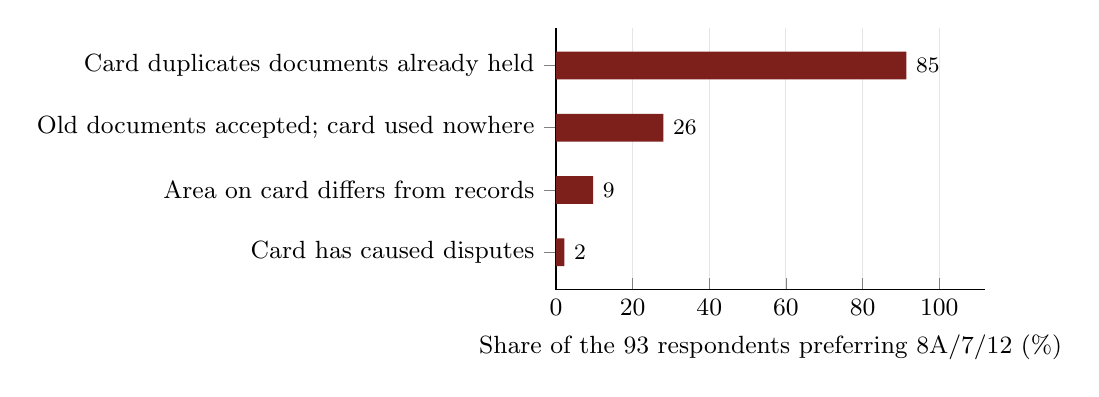
\begin{tikzpicture}
\begin{axis}[
    xbar, bar width=10pt,
    width=0.58\textwidth, height=4.9cm,
    xmin=0, xmax=112, xtick={0,20,40,60,80,100},
    xlabel={Share of the 93 respondents preferring 8A/7/12 (\%)},
    ytick={1,...,4}, y dir=reverse, enlarge y limits={abs=0.6},
    yticklabels={
        Card duplicates documents already held,
        Old documents accepted; card used nowhere,
        Area on card differs from records,
        Card has caused disputes},
    yticklabel style={font=\small},
    xticklabel style={font=\small}, xlabel style={font=\small},
    axis x line*=bottom, axis y line*=left,
    xmajorgrids, major grid style={draw=black!10},
    nodes near coords, point meta=explicit symbolic,
    nodes near coords style={font=\footnotesize, anchor=west},
]
\addplot[fill=oldorange, draw=none] coordinates
    {(91.4,1)[85] (28.0,2)[26] (9.7,3)[9] (2.2,4)[2]};
\end{axis}
\end{tikzpicture}
\end{document}
